% einleitung/einleit.tex
% Motivation
%
% Ausarbeitung zur Diplomarbeit Nr. 2035 - "Erzeugung und Evaluierung 
% von Oktalbaumstrukturen als Schnittstelle zu CAD-Programmen"
%
% Autor: Stefan Mahler 2002
%   Universitaet Stuttgart, SgS
% Betreuer: Ralf Mundani

\chapter{Einleitung}

%Aufgabenstellung was?
%Motivation warum?
%
%Wichtigkeit der Schnittstelle zu CAD-Programmen
%
%CAD === ??? ===> Simulation
%         /\\
%       Octree

In den letzten Jahrzehnten hat sich das rechnergest"utzte Entwickeln neuer
Produkte durchgesetzt. So ist heutzutage das CAD z.B. aus der 
Automobilindustrie nicht mehr wegzudenken. 
Neben dem Modellieren kommt auch der Simulation und Visualisierung 
der daraus resultierenden physikalischen Zusammenh"ange eine gro"se Bedeutung 
zu. Mit Hilfe der Simulation k"onnen Szenarien nachvollzogen, optimiert bzw. 
verstanden werden. Computersimulationen finden in unterschiedlichsten
Bereichen eine breite Anwendung (vgl. \cite{gl_modell_sim}). Einen besonders 
hohen Stellenwert haben Simulationen in Bereichen, in denen die Simulationen 
auf physikalischen Modellen basieren. Beispiele hierf"ur sind der Automobilbau 
(Str"omungssimulation, Crashtests) oder das Bauingeneurwesen (H"auser in 
Erdbebengebieten, Br"uckenstatiken). Simulationen sind h"aufig aus ethischen 
(Belastbarkeit in Extremsituationen) oder betriebswirtschaftlichen 
(Kostenreduktion, Verminderung des Zeitaufwands) Gesichtspunkten vorteilhaft. 
Unter Umst"anden ist die Alternative -- ein mechanisches Modell -- auch gar 
nicht m"oglich. So k"onnen Computersimulationen z.B. helfen, Schw"achen in 
einem neuentworfenen Produkt schneller und kosteng"unstiger zu erkennen als 
das vielleicht an einem mechanischen Modell m"oglich w"are. 

Die Vorteile der Nutzung des Computers zur Modellierung, Simulation und 
Visualisierung innerhalb verschiedenartigster Anwendungsgebiete
liegen auf der Hand. Nat"urlich ist auch eine integrierte L"osung 
anzustreben. Es sollte also ein gemeinsames Modell f"ur Simulation
und Visualisierung genutzt werden k"onnen. Die Nutzung nur \emph{einer}
Datenbasis vermeidet Inkonsistenzen innerhalb der Daten. M"uhsame
und zeitaufw"andige Neueingaben der Produktdaten f"ur Simulation
und Visualisierung werden unn"otig. Doch genau hier liegt das Problem
f"ur einen integrierten Prozess, der sowohl Modellierung als auch
Simulation und Visualisierung umfasst.

Zur Datenhaltung in zur Modellierung verwendeten CAD-Systemen kommen h"aufig
oberfl"achenorientierte Datenmodelle oder das CSG-Modell zum Einsatz. 
Diese erscheinen auch hierf"ur am leistungsf"ahigsten, sind jedoch f"ur die
Simulation ungeeignet. Zur Simulation ist eine Datenbasis als diskretisiertes 
Volumenmodell notwenig. \cite{diss_oct} zeigt, dass die Oktalbaumstruktur 
als effiziente L"osung dieses Problems genutzt werden kann.
Abbildung \ref{abb_schnittstelle_oct} stellt diese Zusammenh"ange schematisch 
dar.

\diabeg
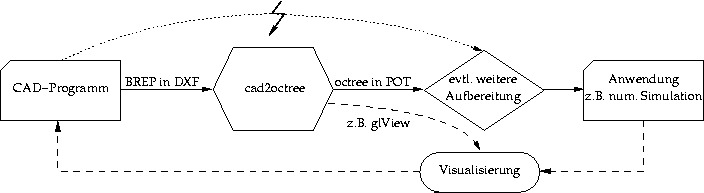
\includegraphics[width=\linewidth]{schnittstelle_oct}
\caption{Octree als Schnittstellte zu CAD-Programmen}
\label{abb_schnittstelle_oct}
\diaend

Thema dieser Arbeit ist, ein Verfahren zu entwickeln, welches aus gegebenen
CAD-Daten, also einem Oberfl"achenmodell, die zugeh"orige Oktalbaumstruktur
generiert.

Kapitel \ref{geombeschr} gibt einen "Uberblick "uber die
wichtigsten Formen zur Geometriebeschreibung. Besondere Aufmerksamkeit
werden dabei den raumpartitionierenden Strukturen, insbesondere dem Octree, 
gegeben. Einen weiteren Schwerpunkt in diesem Kapitel bilden Splines, die 
als Beschreibungsmittel f"ur Freiformfl"achen dienen.

F"ur den Import des CAD-Modells wird auf das DXF-Format zur"uckgegriffen. 
Weshalb die Entscheidung auf dieses Format fiel und welche Eigenschaften es 
besitzt, ist Inhalt von Kapitel \ref{eval}. 

Im Kapitel \ref{algo} werden grundlegende Verfahren zur Bearbeitung 
geometrischer Gebilde, wie Schnitt zweier Geraden im 3-Dimensionalen oder 
der Punkt-in-Ebene-Test erl"autert. Es werden die f"ur die Generierung 
der Oktalbaumstruktur aus dem CAD-Modell zugrundeliegenden Algorithmen 
beschrieben. 
F"ur manche Teilprobleme k"onnen unterschiedliche Algorithmen verwendet 
werden. Vor- und Nachteile der verschiedenen L"osungsalgorithmen werden 
gegen"ubergestellt.

Das im Rahmen dieser Arbeit erstellte Programm wird in unterschiedlichen 
Szenarien auf seine Effizienz untersucht. Die Ergebnisse sind neben 
implementierungtechnischen Details im Kapitel \ref{impl} dargestellt.

Abschlie"send fasst Kapitel \ref{fazit} die erzielten Ergebnisse zusammen
und zeigt f"ur das entwickelte Programm Erweiterungsm"oglichkeiten.

An dieser Stelle m"ochte ich mich bei Prof. Dr. Hans-Joachim Bungartz 
bedanken, der mir erm"oglichte, dieses interessante Thema in dieser 
Diplomarbeit zu bearbeiten.
Besonderen Dank geht an meinen Betreuer Dipl. Inf. Ralf-Peter Mundani f"ur 
die vielen guten Ratschl"age, die moralische Unterst"utzung, das 
Korrekturlesen, die Zeit, die er sich genommen hat, um mit mir offene 
Fragen und Probleme zu er"ortern und dass er mir den Oktalbaumbetrachter 
\texttt{glView} zur Verf"ugung stellte. 

%% End of Document